\chapter{Perancangan}
\label{chap:perancangan}

\section{Perancangan Fisik Basis Data}

\subsection{Perancangan Tabel}
\label{sec:perancngan tabel}

Tabel data yang akan digunakan untuk sistem rekomendasi program studi Universitas Katolik Parahyangan sesuai diagram ERD pada gambar \ref{fig:diagram erd} akan dirancang sesuai pada tabel beriku :

\begin{enumerate}
    \item Jurusan SMA
    
        \begin{table}[H]
            \centering
            \begin{tabular}{|c|p{4cm}|p{4cm}|p{4cm}|}
                \hline
                No & Nama Atribut & Tipe Data & Keterangan \\
                \hline
                1 & id\_jurusan & INT & NOT NULL, Primary Key \\
                \hline
                2 & nama\_jurusan & VARCHAR(25) & NOT NULL\\
                \hline
            \end{tabular}
            \caption{Perancangan Tabel jurusan\_sma}
            \label{tab:perancangan tabel jurusan sma}
        \end{table}
    
    \item Fakultas
    
        \begin{table}[H]
            \centering
            \begin{tabular}{|c|p{4cm}|p{4cm}|p{4cm}|}
                \hline
                No & Nama Atribut & Tipe Data & Keterangan \\
                \hline
                1 & id\_fakultas & INT & NOT NULL, Primary Key \\
                \hline
                2 & nama\_fakultas & VARCHAR(50) & NOT NULL\\
                \hline
            \end{tabular}
            \caption{Perancangan Tabel fakultas}
            \label{tab:perancangan tabel fakultas}
        \end{table}
        
    \item Program Studi
        
        \begin{table}[H]
            \centering
            \begin{tabular}{|c|p{4cm}|p{4cm}|p{4cm}|}
                \hline
                No & Nama Atribut & Tipe Data & Keterangan \\
                \hline
                1 & id\_program\_studi & INT & NOT NULL, Primary Key \\
                \hline
                2 & nama\_program\_studi & VARCHAR(50) & NOT NULL \\
                \hline
                3 & id\_fakultas & INT & NOT NULL, Foreign Key dari fakultas \\
                \hline
                4 & id\_jurusan & INT & NOT NULL, Foreign Key dari jurusan\_sma \\
                \hline
            \end{tabular}
            \caption{Perancangan Tabel program\_studi}
            \label{tab:perancangan tabel program studi}
        \end{table}
        
    \item Mahasiswa
        
        \begin{table}[H]
            \centering
            \begin{tabular}{|c|p{4cm}|p{4cm}|p{4cm}|}
                \hline
                No & Nama Atribut & Tipe Data & Keterangan \\
                \hline
                1 & id\_mahasiswa & INT & NOT NULL, Primary Key \\
                \hline
                2 & NPM & VARCHAR(10) & NOT NULL \\
                \hline
                3 & IPK & DOUBLE & NOT NULL\\
                \hline
                4 & id\_jurusan & INT & NOT NULL, Foreign Key dari jurusan\\
                \hline
                5 & id\_program\_studi & INT & NOT NULL, Foreign Key  dari program\_studi \\
                \hline
            \end{tabular}
            \caption{Perancangan Tabel mahasiswa}
            \label{tab:perancangan tabel mahasiswa}
        \end{table}
        
    \item Mata Pelajaran
        
        \begin{table}[H]
            \centering
            \begin{tabular}{|c|p{4cm}|p{4cm}|p{4cm}|}
                \hline
                No & Nama Atribut & Tipe Data & Keterangan \\
                \hline
                1 & id\_mata\_pelajaran & INT & NOT NULL, Primary Key \\
                \hline
                2 & nama\_mata\_pelajaran & VARCHAR(20) & NOT NULL\\
                \hline
            \end{tabular}
            \caption{Perancangan Tabel mata\_pelajaran}
            \label{tab:perancangan tabel mata pelajaran}
        \end{table}
        
    \item Nilai
    
        \begin{table}[H]
            \centering
            \begin{tabular}{|c|p{4cm}|p{4cm}|p{4cm}|}
                \hline
                No & Nama Atribut & Tipe Data & Keterangan \\
                \hline
                1 & id\_nilai & INT & NOT NULL, Primary Key \\
                \hline
                2 & id\_mata\_pelajaran & INT & Foreign Key dari mata\_pelajaran \\
                \hline
                3 & id\_mahasiswa & INT & NOT NULL, Foreign Key dari mahasiswa \\
                \hline
                4 & 101 & DOUBLE & Nilai kelas 10 semester 1 \\
                \hline
                5 & 102 & DOUBLE & Nilai kelas 10 semester 2 \\
                \hline
                6 & 111 & DOUBLE & Nilai kelas 11 semester 1 \\
                \hline
                7 & 112 & DOUBLE & Nilai kelas 11 semester 2 \\
                \hline
                8 & AVG & DOUBLE & Rata-rata nilai \\
                \hline
            \end{tabular}
            \caption{Perancangan Tabel nilai}
            \label{tab:perancangan tabel nilai}
        \end{table}
\end{enumerate}

\section{Perancangan Algoritma}
\label{sec:perancangan algoritma}

Pada subab ini akan berisikan perancangan algoritma yang digukan pada sistem. Sistem menggunakan beberapa algoritma seperti K-Means untuk membuat kelompok mahasiswa yang memiliki karakteriksi yang sama dengan calon mahasiswa, Pearson Correlation Coefficient untuk menghitung kesamaan atau similaritas, dan User-base Collaborative Filtering untuk menghitung prediksi nilai IPK.

\subsection{K-Means}

\begin{algorithm}
\caption{test}
\end{algorithm}

\subsection{Pearson Correlation Coefficient}

\subsection{User-based Collaborative Filtering}

\section{Perancangan Antar Muka}
\label{sec:perancangan antar muka}

Pada subab ini akan berisikan perancangan antar muka untuk sistem rekomendasi, berikut merupakan hasil perancangan :

\begin{enumerate}
    \item Halaman index saat siswa/i mengakses sistem
    
    \begin{figure}[H]
        \centering
        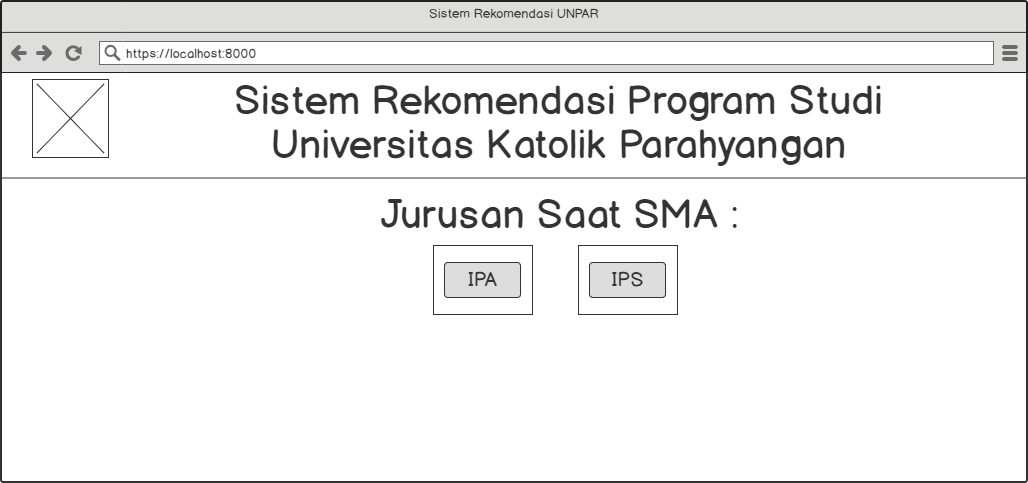
\includegraphics[width = 12cm, height =8 cm]{doc/DokumenSkripsi/Gambar/gambar41.png}
        \caption{Halaman Index Sistem}
        \label{fig:gambar41}
    \end{figure}
    
    \item Halaman pengisian nilai siswa/i IPA
    
    \begin{figure}[H]
        \centering
        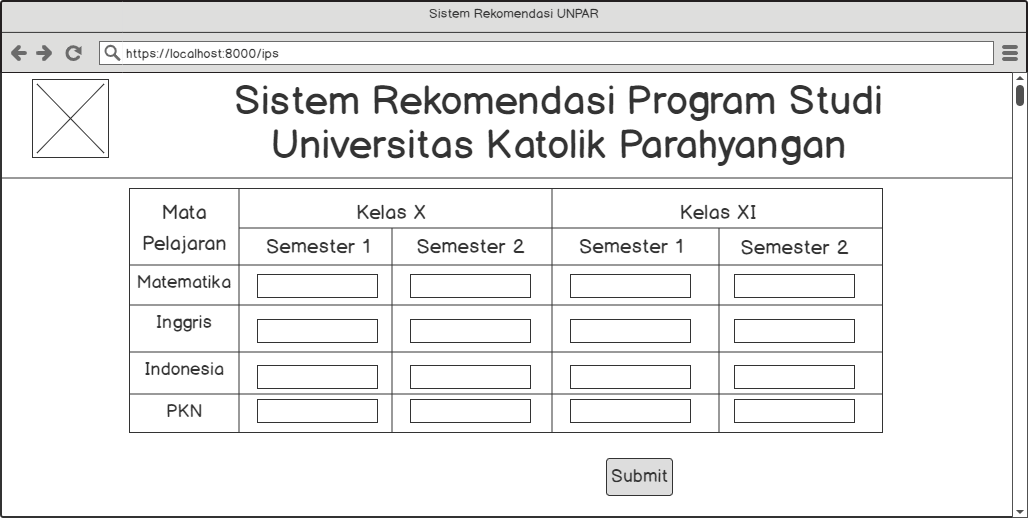
\includegraphics[width = 12cm, height =8 cm]{doc/DokumenSkripsi/Gambar/gambar42.png}
        \caption{Halaman Pengisian Nilai IPA}
        \label{fig:gambar42}
    \end{figure}
    
    \item Halaman pengisian nilai siswa/i IPS
    
    \begin{figure}[H]
        \centering
        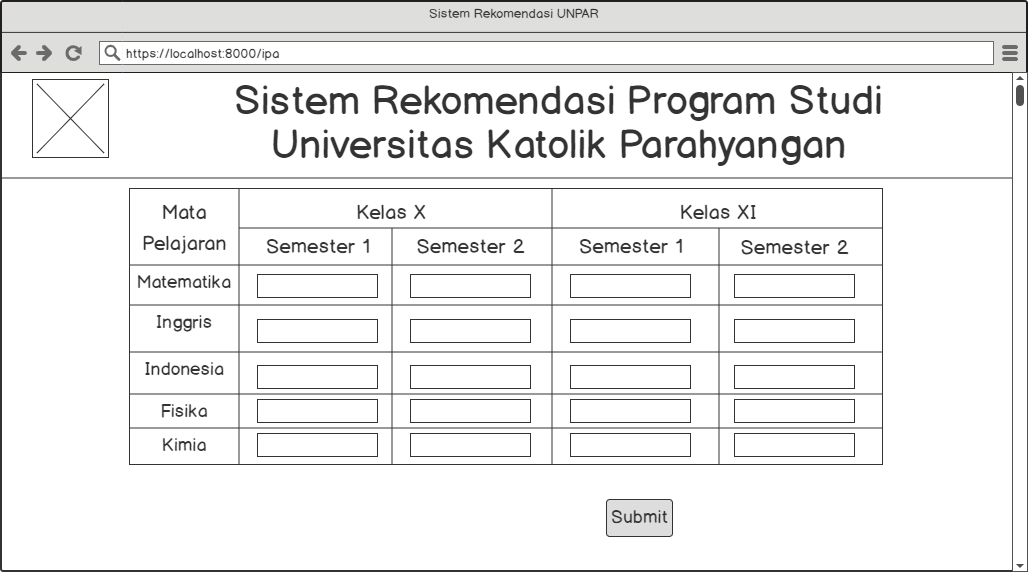
\includegraphics[width = 12cm, height =8 cm]{doc/DokumenSkripsi/Gambar/gambar43.png}
        \caption{Halaman Pengisian Nilai IPS}
        \label{fig:gambar43}
    \end{figure}
    
    \item Halaman hasil rekomendasi
    
    \begin{figure}[H]
        \centering
        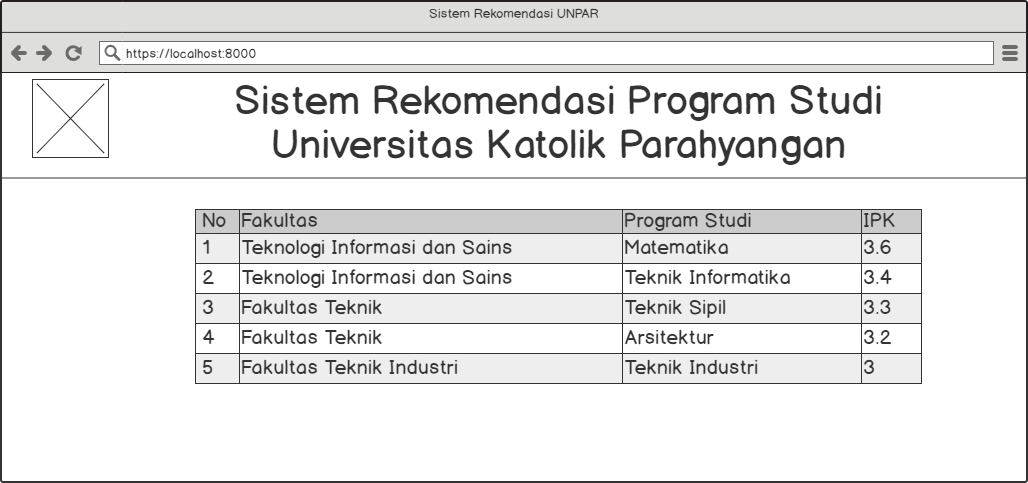
\includegraphics[width = 12cm, height =8 cm]{doc/DokumenSkripsi/Gambar/gambar44.png}
        \caption{Halaman Hasil Rekomendasi}
        \label{fig:gambar44}
    \end{figure}
\end{enumerate}